\documentclass[xcolor=dvipsnames, noamsthm]{beamer}
%THEME AUSWÄHLEN
\usetheme{default}      

%PAKETE LADEN 
\usepackage[english]{babel}
\usepackage[utf8]{inputenc}
\usepackage{amsthm, amsmath, graphicx, amssymb}
\newcommand{\thickbar}[1]{\mathbf{\bar{\text{$#1$}}}}
\usepackage{comment}
\usepackage[T1]{fontenc}
\usepackage{lmodern} % font 
\usefonttheme[onlymath]{serif} % Aendert den Mathefont zur serif variante 
\usepackage{bm}       % bm fuer bold math mit gutem spacing
\usepackage{caption}
\captionsetup{justification   = raggedright,
	singlelinecheck = false}

\usepackage{subcaption} %two figs side-by-side

%online table generator
\usepackage{multirow}
\usepackage[normalem]{ulem}
\useunder{\uline}{\ul}{}
%BIBTEX 
\usepackage[round]{natbib}

\usepackage{multicol} % multiple cols with items



\usepackage{tikz}

\newcommand{\bluecheck}{}%
\DeclareRobustCommand{\greencheck}{%
	\tikz\fill[scale=0.4, color=green]
	(0,.35) -- (.25,0) -- (1,.7) -- (.25,.15) -- cycle;%
}



\renewcommand{\bibsection}{\subsubsection*{\bibname } } %OMIT REFERNCES FROM TOC
\bibliographystyle{plainnat}

\setbeamertemplate{caption}[numbered]

%FARBE DEFINIEREN
\definecolor{Teal}{HTML}{000080} %Alternativ: Einfach den HTML Code Ändern. Aber änder nicht das Teal, das ist ueberall drin! 

%COLOR THEME UMSTELLEN
\usecolortheme[named=Teal]{structure} %ersetzt das ganze standard blau gegen Teal 
%FOOTLINE EINSTELLEN
\makeatletter %footline ändern. 
\setbeamertemplate{footline}
% remove footline from title page
{
	    \ifnum \theframenumber=1
	% This is the title frame, do nothing
	
	\else
{
	\leavevmode%
	\hbox{%
	\begin{beamercolorbox}[wd=.60\paperwidth,ht=2.25ex,dp=1ex,left]{title in head/foot}\textcolor{Black}{\inserttitle}\hspace{0em}
	\end{beamercolorbox}}%
		\begin{beamercolorbox}[wd=.15\paperwidth,ht=2.25ex,dp=1ex,center]{author in head/foot}%
			\usebeamerfont{author in head/foot}{
			\insertsectionnavigationhorizontal{.30\paperwidth}{}{}} %alternativ: 65. Kannst du runterstellen wenn du platz brauchst 
		\end{beamercolorbox}%
  \begin{beamercolorbox}[wd=.4\paperwidth,ht=2.25ex,dp=1ex,center]{date in head/foot}%

 

{	\textcolor{Black}{\insertframenumber{} / \inserttotalframenumber}\usebeamerfont{page number in head/foot} }
\end{beamercolorbox}}%

    \fi
}
	\vskip0pt%
\makeatother
%HEADLINE   %headline ändern 
\makeatletter
\setbeamertemplate{headline}
{
	\leavevmode
	\begin{beamercolorbox}[wd=.975\paperwidth,ht=3.8ex,dp=0ex,right]{framesubtitle in head}
		\hspace{20em}{\insertframesubtitle}
	\end{beamercolorbox}
}
\makeatother

%REDEFINE FRAMETITLE: FRAMESUBTITLE AUS DEM MAINFRAME RAUS
\makeatletter
\setbeamertemplate{frametitle}{
	\ifbeamercolorempty[bg]{frametitle}{}{\nointerlineskip}%
	\@tempdima=\textwidth%
	\advance\@tempdima by\beamer@leftmargin%
	\advance\@tempdima by\beamer@rightmargin%
	\begin{beamercolorbox}[sep=0.3cm,left,wd=\the\@tempdima]{frametitle}
		\usebeamerfont{frametitle}%
		\vbox{}\vskip-1ex%
		\if@tempswa\else\csname beamer@ftecenter\endcsname\fi%
		\strut\insertframetitle\strut\par%
		{%
			\ifx\@empty%
			\else%
			{\usebeamerfont{framesubtitle}\usebeamercolor[fg]{framesubtitle}\strut\par}%
			\fi
		}%
		\vskip-1ex%¸
		\if@tempswa\else\vskip-.3cm\fi% set inside beamercolorbox... evil here...
	\end{beamercolorbox}%
}
\makeatother

%NAVIGATION AUS
\setbeamertemplate{navigation symbols}{}
%FONT: TITLEPAGE ÄNDERN
\setbeamerfont{title}{size=\LARGE,series=\bfseries,parent=structure}
\setbeamerfont{subtitle}{size=\large,series=\normalfont,parent=structure}
\setbeamerfont{author}{size=\normalsize,series=\normalfont,parent=structure}
\setbeamerfont{institute}{size=\scriptsize,series=\normalfont,parent=structure}
\setbeamerfont{date}{size=\scriptsize,series=\normalfont,parent=structure}


%FARBEN EINSTELLEN
\setbeamercolor{title}{fg=black}
%ITEMIZE
\setbeamertemplate{itemize item}[square]
\setbeamertemplate{itemize subitem}[triangle]
\setbeamertemplate{itemize subsubitem}[circle]
\colorlet{shadecolor}{gray!40}





%HYPERREF
\hypersetup{
	colorlinks = true,
	linkbordercolor = {white}, 
	linkcolor       = {Teal}, 
	citecolor =    {black}
}

%EMPHASIZE: Falls du gerne emphasize in irgend einer Farbe hättest einfach das fg=black durch fg=Teal ersetzen
\setbeamercolor{emph}{fg=black}
\renewcommand<>{\emph}[1]{%
	{\usebeamercolor[fg]{emph}\only#2\itshape{}#1}%
}

%AMSMATH 
%REMARK; THM; DEF REDEFINIEREN
%REMARK
\newtheoremstyle{remark}%
{3pt}% Space above
{3pt}% Space below 
{\normalfont}% Body font
{}% Indent amount
{\itshape\color{Teal}}% Theorem head font
{.}% Punctuation after theorem head
{.5em}% Space after theorem head 
{}% Theorem head spec (can be left empty, meaning ‘normal’)
%THEOREM
\newtheoremstyle{thm} % name
{3pt}    	                 % Space above
{3pt}                        % Space below
{\itshape}                   % Body font
{}                           % Indent amount
{\bfseries\color{Teal}}                   % Theorem head font
{.}                          % Punctuation after theorem head
{.5em}                       % Space after theorem head
{\thmname{#1}\thmnumber{ #2}\thmnote{ \normalfont (#3)}}  % Theorem head spec (can be left empty, meaning ‘normal’)
%DEFINITION
\newtheoremstyle{def} % name
{3pt}    	                 % Space above
{3pt}                        % Space below
{\normalfont}                   % Body font
{}                           % Indent amount
{\bfseries\color{Teal}}                   % Theorem head font
{.}                          % Punctuation after theorem head
{.5em}                       % Space after theorem head
{\thmname{#1}\thmnumber{ #2}\thmnote{ \normalfont (#3)}}  % Theorem head spec (can be left empty, meaning ‘normal’)


\theoremstyle{remark}
\newtheorem{remark}{Remark}
\theoremstyle{thm}
\newtheorem{thm}{Theorem}
\theoremstyle{def}
\newtheorem{definition}{Definition}

%TITLE
\title{\textcolor{Teal}{On Using Metropolis-Hastings to Analyze Democratic Support}}
\subtitle{Final Paper for Advanced Quantitative Methods}
\author{Tobias Stenzel}
\institute{Chair of Quantitative Methods in the Social Sciences, Prof. Gschwend}
\date{\today}
%FIX CITATION
\makeatletter
\let\@mycite\@cite
\def\@cite#1#2{{\hypersetup{linkcolor=Black}[{#1\if@tempswa , #2\fi}]}}
\makeatother

%DEF: framesubtitle 
\def\insertframesubtitle{}

\begin{document}
\begin{frame} %TITLEPAGE 
\maketitle
\end{frame}


\begin{comment}
\section{Conclusion}
\begin{frame}\frametitle{Some math}
	\begin{align} 
Y_t &= A_0 Y_t + A_1 Y_{t-1} + \varepsilon_t \tag{VAR(1)} \\
Y_t &= (I- A_0)^{-1}  \Big( A_1 Y_{t-1} + \varepsilon_t \Big) \label{eq:eins} 
\intertext{	In Equation \ref{eq:eins}, define }
\nu_t &\equiv (I- A_0)^{-1} \varepsilon_t, \quad B_1 \equiv (I- A_0)^{-1} A_1 \nonumber 
		\end{align}
	\begin{remark}
	Ich habe serif Mathe genommen. Genau wie bei BB. Kann man ändern.
	\end{remark} 
Remark Farbig machen? 
\end{frame}
\end{comment}





\begin{frame}\frametitle{Panel Data on Public Democratic Support $y_{ikt}$}


	\cite{Claassen2019estimating} estimation, \cite{Claassen2020support, Claassen2020mood} DV and IV


	
\begin{figure}
	\centering
	\begin{subfigure}[b]{0.85\textwidth}
		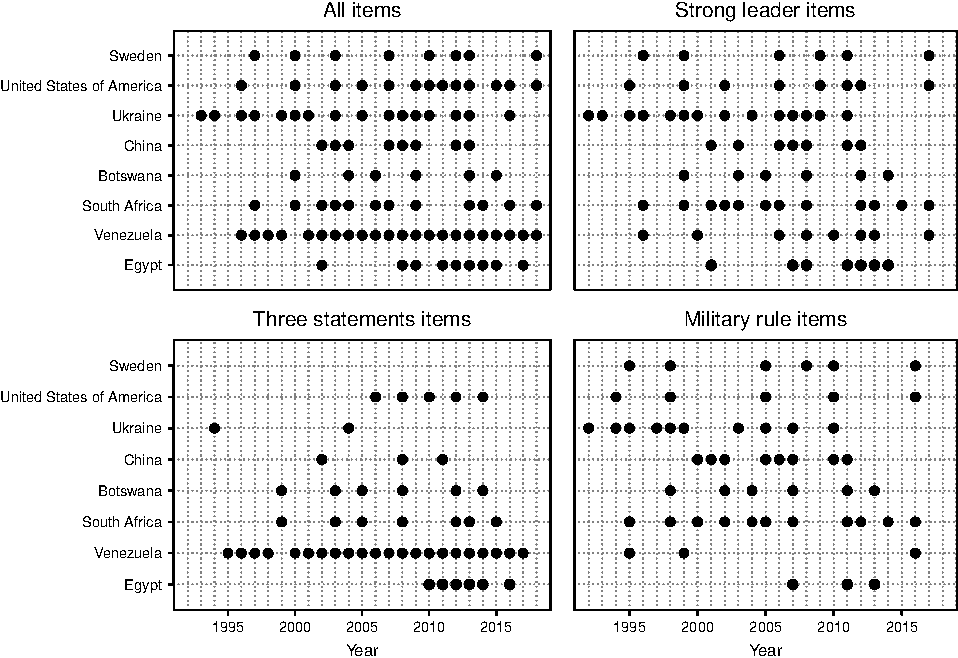
\includegraphics[width=8cm]{figs/sparse-data-1.pdf}

	\end{subfigure}
	

	
	%\caption{Community data vs. baseline models}
\end{figure}



 
\end{frame}



\begin{frame}\frametitle{Model Estimated by MH Algorithm}
\begin{gather*}

		
	y_{ikt} \sim \text{Binomial}(s_{ikt}, \pi_{ikt})\\
	
	\pi_{ikt} \sim \text{Beta}(\alpha_{ikt}, \pi_{ikt})\\
	
	\alpha_{ikt} = \phi \eta_{ikt}\\
	
	\beta_{ikt} = \phi (1 - \eta_{ikt})\\
	
	\eta_{ikt} = \text{logit}^{-1}(\lambda_k + \delta_{ik} + \theta_{it})\\
	
	\lambda_k = \mathcal{N}(\mu_{\lambda}, \sigma_{\lambda}^2)\\
		
	\delta_k = \mathcal{N}(0, \sigma_{\delta}^2)\\
		
	\theta_{it} = \mathcal{N}(\theta_{i,t-1}, \sigma_{\theta}^2)	
\end{gather*}


\end{frame}



\begin{frame}\frametitle{Varying MH Iteration Numbers}
	\begin{figure}
		\centering
		\begin{subfigure}[b]{0.95\textwidth}
			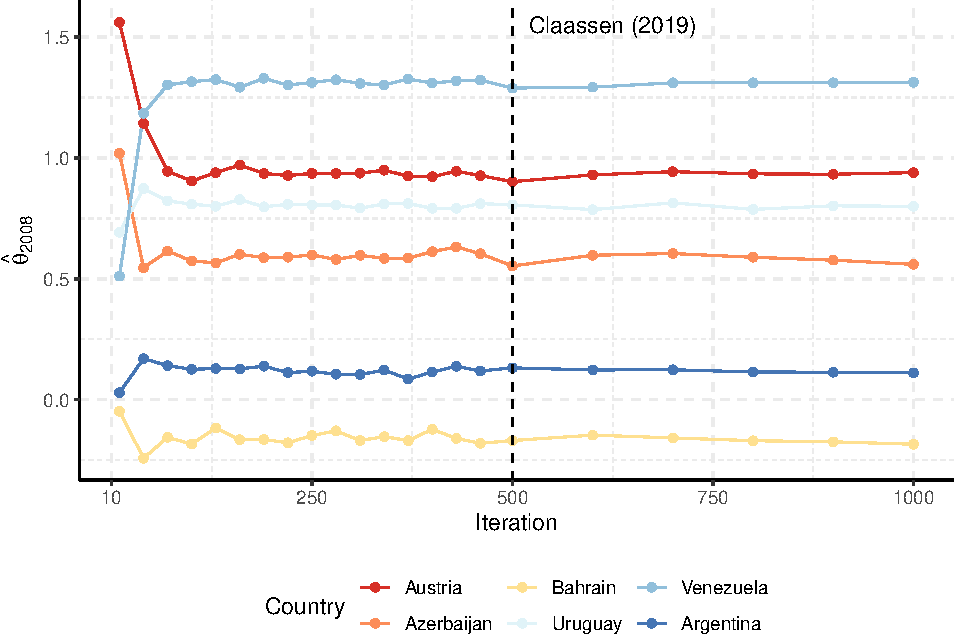
\includegraphics[width=10cm]{figs/niter-1.pdf}

		\end{subfigure}
	\end{figure}	
\end{frame}



\begin{frame}\frametitle{Old vs. Updated Data (27 vs. 30 years)}
	
	
	\begin{figure}
		\centering
		\begin{subfigure}[b]{0.95\textwidth}
			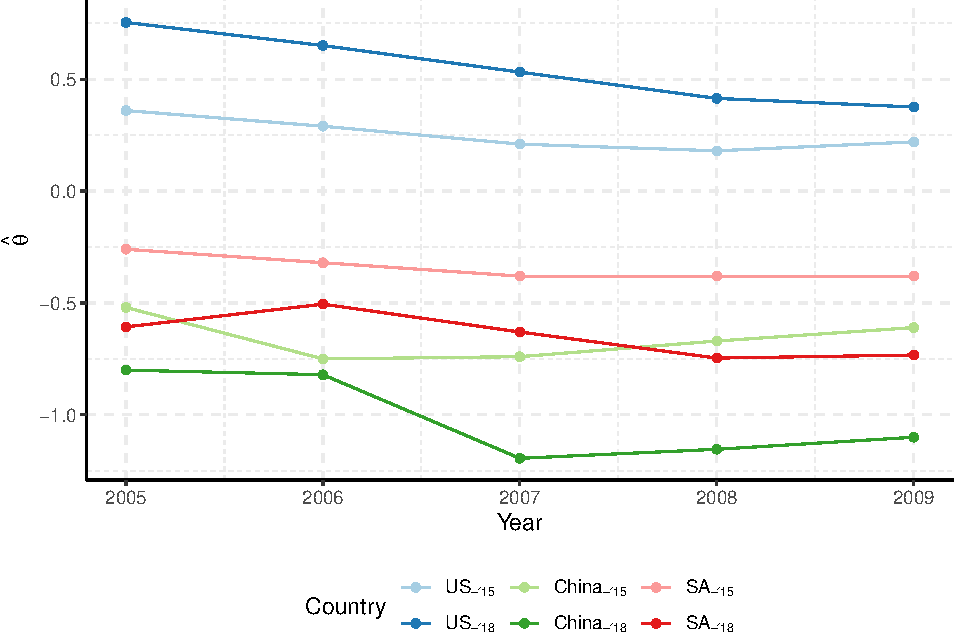
\includegraphics[width=10cm]{figs/data-1.pdf}

		\end{subfigure}
		
		
		
		%\caption{Community data vs. baseline models}
	\end{figure}
	
	
	
	
\end{frame}
















%\section{References}
\section*{} 
\begin{frame}\frametitle{References} %REF
\framesubtitle{}
\scriptsize{\bibliography{bib_lib}}
\end{frame}

\end{document}
